

%% This template can be used to write a paper for
%% Computer Physics Communications using LaTeX.
%% For authors who want to write a computer program description,
%% an example Program Summary is included that only has to be
%% completed and which will give the correct layout in the
%% preprint and the journal.
%% The `elsarticle' style is used and more information on this style
%% can be found at 
%% http://www.elsevier.com/wps/find/authorsview.authors/elsarticle.
%%
%%
%\documentclass[preprint,12pt]{elsarticle}
%\documentclass[preprint,12pt]{elsarticle}
%\documentclass[a4paper,pra,twocolumn]{revtex4-1}

%% Use the option review to obtain double line spacing
%% \documentclass[preprint,review,12pt]{elsarticle}

%% Use the options 1p,twocolumn; 3p; 3p,twocolumn; 5p; or 5p,twocolumn
%% for a journal layout:
%% \documentclass[final,1p,times]{elsarticle}
 \documentclass[final,twocolumn]{elsarticle}
%% \documentclass[final,3p,times]{elsarticle}
%% \documentclass[final,3p,times,twocolumn]{elsarticle}
%% \documentclass[final,5p,times]{elsarticle}
%% \documentclass[final,5p,times,twocolumn]{elsarticle}




%\usepackage[latin]{babel}
%\usepackage{ltxgrid}
\usepackage{algpseudocode,algorithm}
\algrenewcommand\textproc{\texttt} % function name in typewriter font in algorithm
%\usepackage[ruled,vlined,linesnumbered,resetcount,algochapter]{algorithm}



%\renewcommand{\thealgorithm}{}% disbale the ref numbers 

\usepackage{graphicx}
\usepackage{physics}
\usepackage{comment}
\usepackage{hyperref}
\usepackage{color,soul}


\usepackage{multirow}
\usepackage{tikz}
\usepackage{verbatim}
\usetikzlibrary{arrows}
\usetikzlibrary{calc}


\usepackage{amsmath,amssymb}
\usepackage{graphicx}
\usepackage{physics}
\usepackage{comment}
\usepackage{hyperref}
\usepackage{color,soul}

\newcommand{\da}{\downarrow}
\newcommand{\ua}{\uparrow}
\newcommand{\ad}{\hat{a}^\dagger}
\newcommand{\an}{\hat{a}^{}}
\newcommand{\bd}{\hat{b}^\dagger}
\newcommand{\bn}{\hat{b}^{}}
\newcommand{\sd}{\hat{\sigma}^{+}}
\newcommand{\sn}{\hat{\sigma}^{-}}
\newcommand{\mbf}[1]{\mathbf{#1}}
\newcommand{\dn}{\hat{\Delta}^{}_i}

\newcommand{\az}[1]{{\color{magenta}{#1}}}
\newcommand{\jk}[1]{{\color{red}{#1}}}
\newcommand{\pk}[1]{{\color{blue}{#1}}}

\newcommand{\kb}{\ket{0}\!\bra{0}}
\newcommand{\klb}{\ket{\lambda}\!\bra{0}}
\newcommand{\kbl}{\ket{0}\!\bra{\lambda}}
\newcommand{\klbl}{\ket{\lambda}\!\bra{\lambda}}

\newcommand{\symset}{\mathcal{S}}
\newcommand{\cntset}{\mathcal{P}_N}
\newcommand{\cntsetx}{\mathcal{P}_{N-1}} 
\newcommand{\cntsetxx}{\mathcal{P}_{N-2}} 
\newcommand{\indset}{\mathcal{I}} 
\newcommand{\na}{{\mathcal{N}_{1}}}
\newcommand{\nb}{{\mathcal{N}_{2}}}
\newcommand{\nc}{{\mathcal{N}_{3}}}


\newcommand{\Mbm}{{\mathcal{M}(\beta,m)}}
\newcommand{\Mbmp}{{\mathcal{M}(\beta,m^\prime)}}
\newcommand{\Mgm}{{\mathcal{M}(\gamma,m)}}
\newcommand{\Mgmp}{{\mathcal{M}(\gamma,m^\prime)}}

\newcommand{\maptoN}{{{\mathcal{M}}}_{N-1 \mapsto N}}
\newcommand{\maptoNa}{{\mathcal{M}}_{N-2 \mapsto N-1}}

\newcommand{\pluseq}{\mathrel{+}=}
\newcommand{\str}{$\ast\ast\ast\ast\ast\ast\ast$}

%% Use the option review to obtain double line spacing
%% \documentclass[preprint,review,12pt]{elsarticle}

%% Use the options 1p,twocolumn; 3p; 3p,twocolumn; 5p; or 5p,twocolumn
%% for a journal layout:
%% \documentclass[final,1p,times]{elsarticle}
%% \documentclass[final,1p,times,twocolumn]{elsarticle}
%% \documentclass[final,3p,times]{elsarticle}
%% \documentclass[final,3p,times,twocolumn]{elsarticle}
%% \documentclass[final,5p,times]{elsarticle}
%% \documentclass[final,5p,times,twocolumn]{elsarticle}

%% if you use PostScript figures in your article
%% use the graphics package for simple commands
%% \usepackage{graphics}
%% or use the graphicx package for more complicated commands
%% \usepackage{graphicx}
%% or use the epsfig package if you prefer to use the old commands
%% \usepackage{epsfig}

%% The amssymb package provides various useful mathematical symbols
\usepackage{amssymb}
%% The amsthm package provides extended theorem environments
%% \usepackage{amsthm}

%% The lineno packages adds line numbers. Start line numbering with
%% \begin{linenumbers}, end it with \end{linenumbers}. Or switch it on
%% for the whole article with \linenumbers after \end{frontmatter}.
%% \usepackage{lineno}

%% natbib.sty is loaded by default. However, natbib options can be
%% provided with \biboptions{...} command. Following options are
%% valid:

%%   round  -  round parentheses are used (default)
%%   square -  square brackets are used   [option]
%%   curly  -  curly braces are used      {option}
%%   angle  -  angle brackets are used    <option>
%%   semicolon  -  multiple citations separated by semi-colon
%%   colon  - same as semicolon, an earlier confusion
%%   comma  -  separated by comma
%%   numbers-  selects numerical citations
%%   super  -  numerical citations as superscripts
%%   sort   -  sorts multiple citations according to order in ref. list
%%   sort&compress   -  like sort, but also compresses numerical citations
%%   compress - compresses without sorting
%%
%% \biboptions{comma,round}

% \biboptions{}

%% This list environment is used for the references in the
%% Program Summary
%%
\newcounter{bla}
\newenvironment{refnummer}{%
\list{[\arabic{bla}]}%
{\usecounter{bla}%
 \setlength{\itemindent}{0pt}%
 \setlength{\topsep}{0pt}%
 \setlength{\itemsep}{0pt}%
 \setlength{\labelsep}{2pt}%
 \setlength{\listparindent}{0pt}%
 \settowidth{\labelwidth}{[9]}%
 \setlength{\leftmargin}{\labelwidth}%
 \addtolength{\leftmargin}{\labelsep}%
 \setlength{\rightmargin}{0pt}}}
 {\endlist}

\journal{Computer Physics Communications}








\begin{document}

\begin{frontmatter}

%% Title, authors and addresses

%% use the tnoteref command within \title for footnotes;
%% use the tnotetext command for the associated footnote;
%% use the fnref command within \author or \address for footnotes;
%% use the fntext command for the associated footnote;
%% use the corref command within \author for corresponding author footnotes;
%% use the cortext command for the associated footnote;
%% use the ead command for the email address,
%% and the form \ead[url] for the home page:
%%
%% \title{Title\tnoteref{label1}}
%% \tnotetext[label1]{}
%% \author{Name\corref{cor1}\fnref{label2}}
%% \ead{email address}
%% \ead[url]{home page}
%% \fntext[label2]{}
%% \cortext[cor1]{}
%% \address{Address\fnref{label3}}
%% \fntext[label3]{}

\title{Polaritons: a polynomial scaling code to exactly solve the Holstein-Tavis-Cummings model}

%% use optional labels to link authors explicitly to addresses:
%% \author[label1,label2]{<author name>}
%% \address[label1]{<address>}
%% \address[label2]{<address>}

\author{M. Ahsan Zeb \corref{author}}
\author{Peter G. Kirton}
\author{Jonathan Keeling}
\date{\today}


%\author[a]{First Author\corref{author}}
%\author[a,b]{Second Author}
%\author[b]{Third Author}

\cortext[author]{Corresponding author.\\\textit{E-mail address:} maz3@st-andrews.ac.uk}

\address{SUPA, School of Physics and Astronomy, University of St Andrews, St Andrews, KY16 9SS, United Kingdom}

\begin{abstract}
A submitted program is expected to be of benefit to other physicists or physical chemists, or be an exemplar of good programming practice, or illustrate new or novel programming techniques which are of importance to some branch of computational physics or physical chemistry.

Acceptable program descriptions can take different forms. The following Long Write-Up structure is a suggested structure but it is not obligatory. Actual structure will depend on the length of the program, the extent to which the algorithms or software have already been described in literature, and the detail provided in the user manual.

Your manuscript and figure sources should be submitted through the Elsevier Editorial System (EES) by using the online submission tool at \\
http://www.ees.elsevier.com/cpc.

\end{abstract}

\twocolumn

\begin{comment}
A submitted program is expected to be of benefit to other physicists or physical chemists, or be an exemplar of good programming practice, or illustrate new or novel programming techniques which are of importance to some branch of computational physics or physical chemistry.

Acceptable program descriptions can take different forms. The following Long Write-Up structure is a suggested structure but it is not obligatory. Actual structure will depend on the length of the program, the extent to which the algorithms or software have already been described in literature, and the detail provided in the user manual.

Your manuscript and figure sources should be submitted through the Elsevier Editorial System (EES) by using the online submission tool at \\
http://www.ees.elsevier.com/cpc.

In addition to the manuscript you must supply: the program source code; job control scripts, where applicable; a README file giving the names and a brief description of all the files that make up the package and clear instructions on the installation and execution of the program; sample input and output data for at least one comprehensive test run; and, where appropriate, a user manual. These should be sent, via email as a compressed archive file, to the CPC Program Librarian at cpc@qub.ac.uk.
\end{comment}



\begin{keyword}
%% keywords here, in the form: keyword \sep keyword
keyword1; keyword2; keyword3; etc.

\end{keyword}

\end{frontmatter}


%%
%% Start line numbering here if you want
%%
% \linenumbers

% Computer program descriptions should contain the following
% PROGRAM SUMMARY.

{\bf PROGRAM SUMMARY}
  %Delete as appropriate.

\begin{small}
\noindent
{\em Program Title: Polaritons}                                          \\
{\em Licensing provisions(please choose one): GPLv3}                                   \\
{\em Programming language: Python}                                   \\

%{\em Supplementary material:}                                 \\
  % Fill in if necessary, otherwise leave out.
%Running time: A few seconds up to several tens of minutes, depending on size of underlying Hilbert space.
{\em Nature of problem: Strong light-matter coupling in organic microcavity systems}\\
{\em Solution method:
%The exact numerical solution of Holstein-Tavis-Cummings model,  i.e., a cavity coupled to many two level electronic systems each coupled to a local vibrational mode.
  The code exploits the permutation symmetry of the model for identical molecules
  and works in the permutation symmetric sector of the Hilbert space, which scales only polynomially with the number of molecules. 
  The ground and excited quantum states are efficiently calculated using LOBPCG.
 For the absorption spectrum, either the transition matrix elements
or the two-time correlation function of photon and frequency dependent Green functions are calculated.
 }\\
  %Describe the method solution here.
{\em Additional comments:
  %Provide any additional comments here.
   Two ideas implemented in the code make the use of permutation symmetry really successful.\\
 1. The map between photon and exciton sectors of the basis set that is required to compute the matrix elements of matter-light coupling (and several other quantities) is directly generated in a linear scaling fashion instead of computing it using brute force that scales as the square of the basis size.\\
  2. A unitarily transformed Hamiltonian with an effect of displaced vibrational basis is solved instead. This permits a lower cutoff on the vibrational states and thus further (exponentially) reduces the size of the Hilbert space.\\
These make the solution of thermodynamically large system sizes possible even on a modern laptop.
  %Efficient calc of map: instead of following all the indices and their connections, we can just recognise the pattern they make and directly generate that.
%A unitarily transformed Hamiltonian with an effect of displaced vibrational basis permits a lower cutoff on the vibrational states and thus further reduces the size of the Hilbert space.
%These transformations make the solution of thermodynamically large system sizes possible even on a laptop.
    %To further lower the basis size, the hamiltonian in displaced vibrational basis is solved
    }\\
    
  
\vspace{2cm}




\begin{figure}[t]
\centering
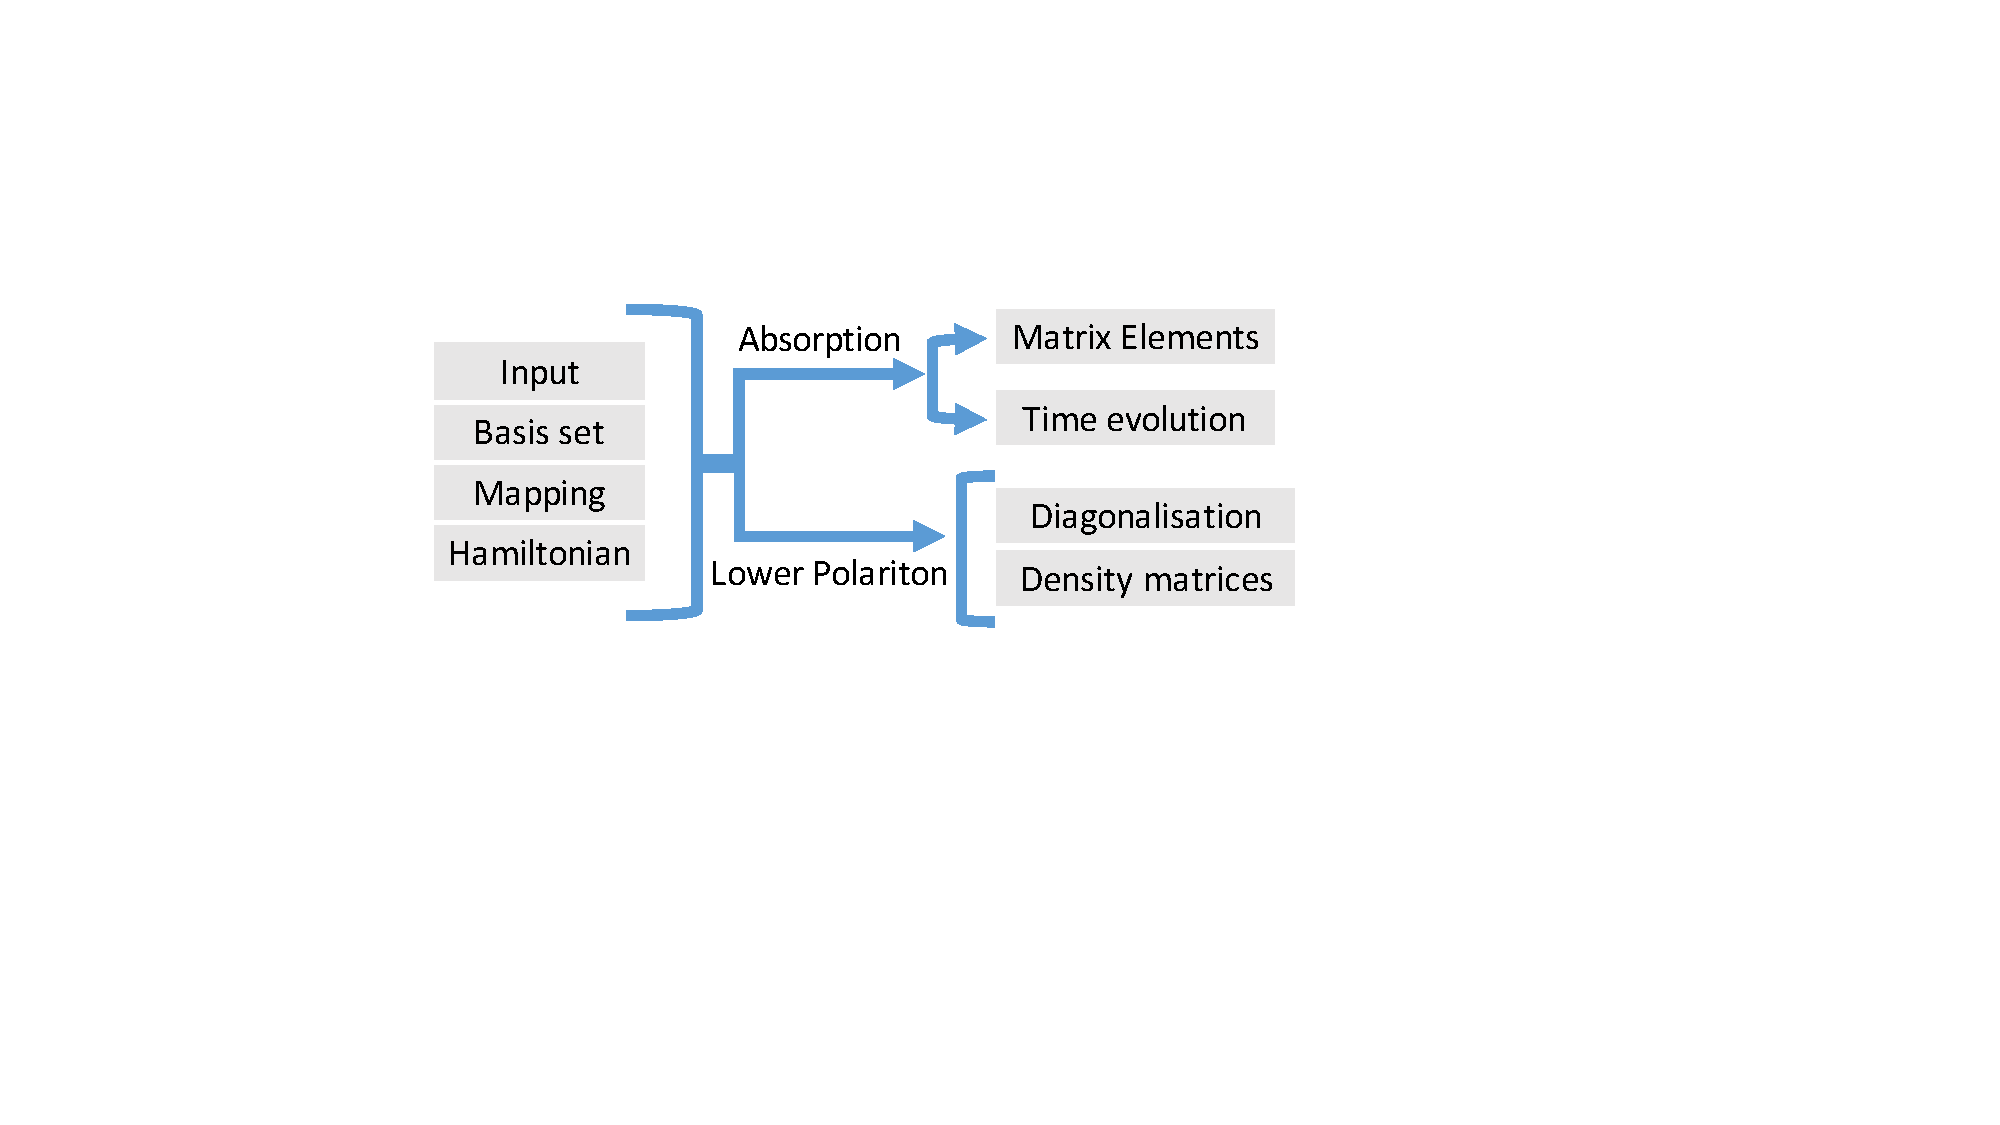
\includegraphics[width=0.8\columnwidth]{flow}
%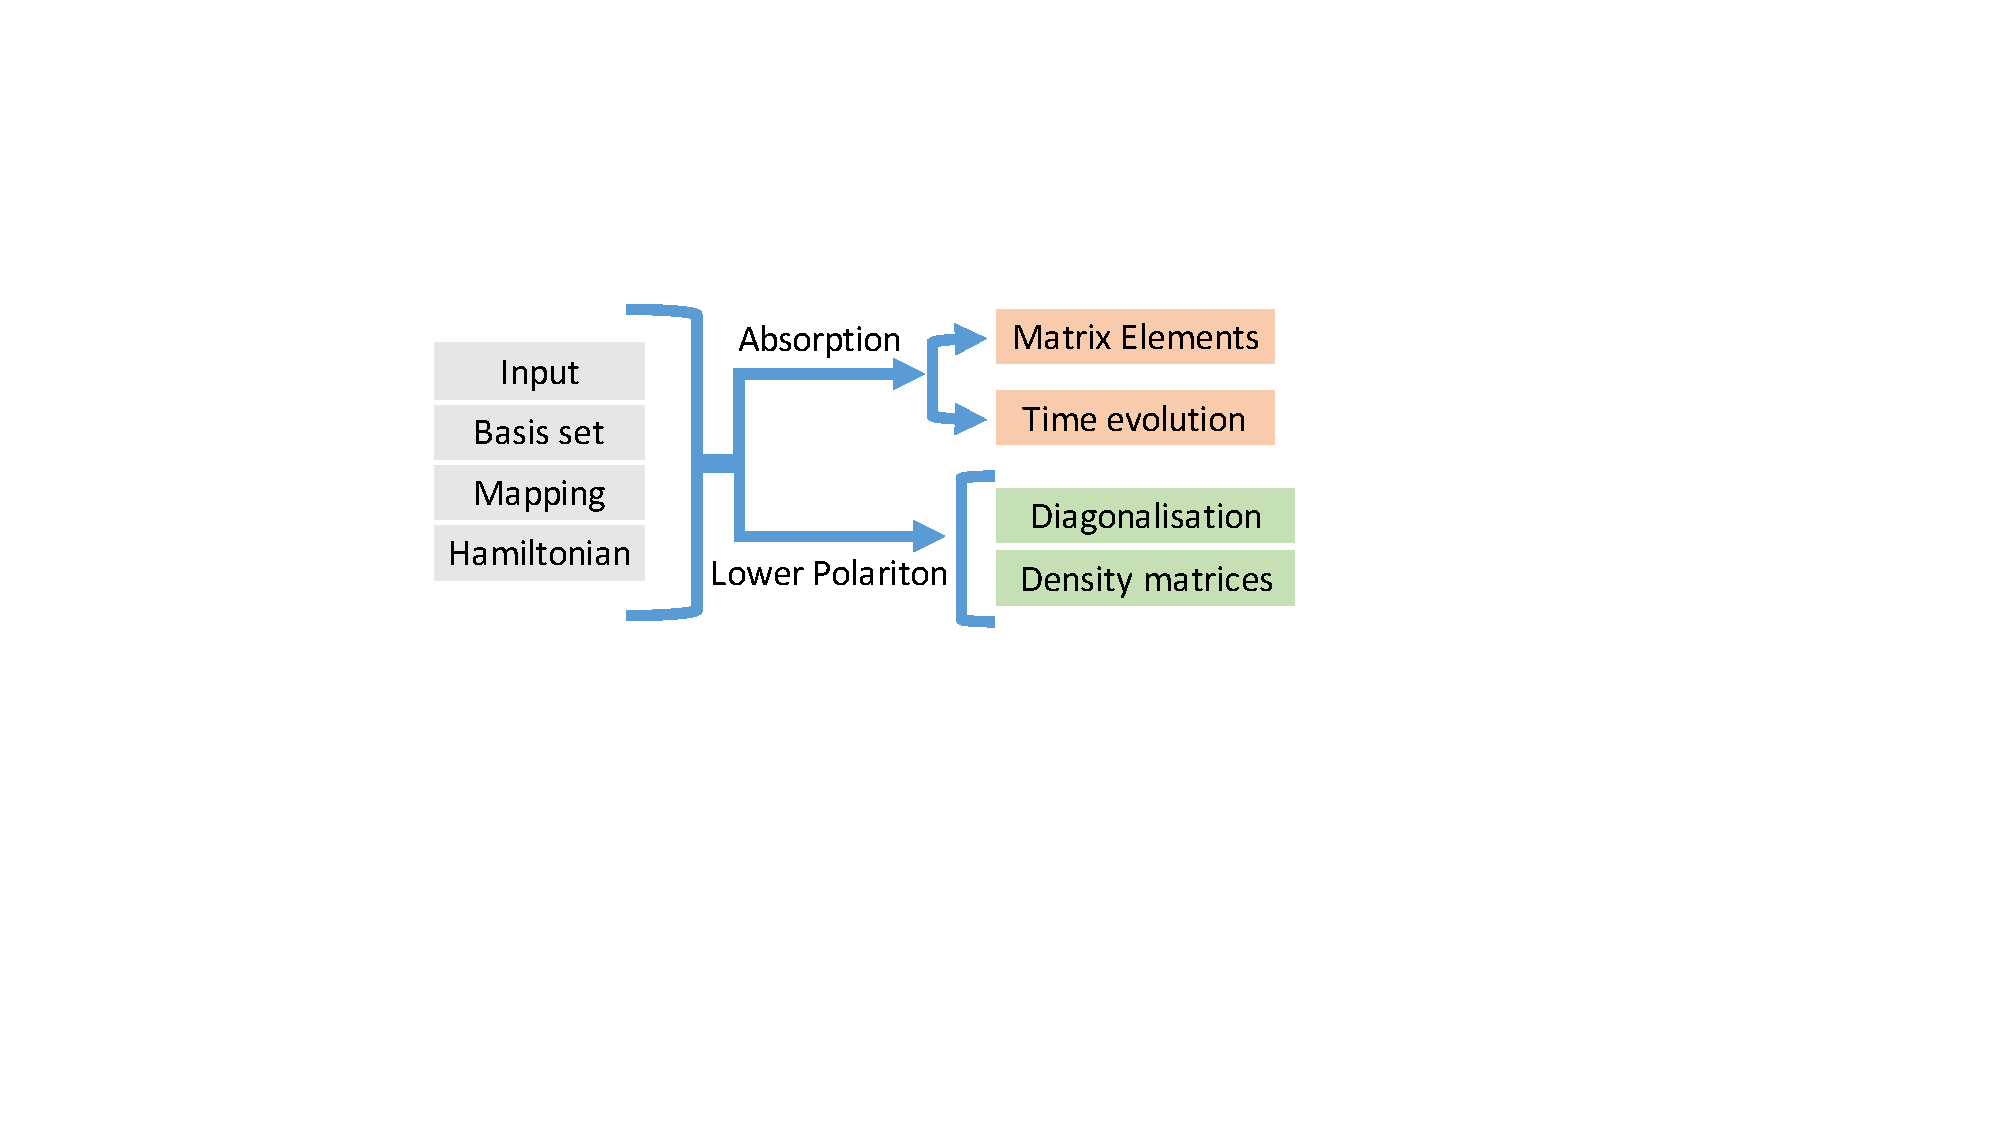
\includegraphics[width=0.8\columnwidth]{flow-c}
\caption{ The sequence of calculations %of various quantities 
that the code performs. %operations.%performs
%First, the input describing the system, type of calculation and required parameters, is read from the input file. Second, for a given $N$ and $M$, the basis set related quantities, like the number of vibrational quanta $N_v$ and permutations $\cntset$ are calculated. Then, the mapping $\maptoN$ and the Hamiltonian matrix elements are calculated that use $N_v$, $\cntset$, and $\maptoN$.
For absorption, either the transition matrix elements are calculated for post-processing or
the two-time correlation function is computed from the time evolution that is used to calculate
the absorption.
%When the lower polariton eigenstate is calculated, the conditional vibrational density matrices can be evaluated for three conditions described in the text/sectionXXX.
 \label{fig:flow}
 }
\end{figure}



\section{workflow/layout/etc}
First the basis,
then,
a map that connects the basis states in the photon and exciton sectors and is used to evaluate the matrix elements of vibrational coupling term and conditional density matrices.






\section{The basis states}

The basis states are (tensor) products of cavity and matter states, the latter consisting of product of electronic and vibrational states of all molecules/\az{sites}. 
The conservation of the number of excitation,
$aa+cc=1$ in this case,
restricts the cavity and electronic basis to only two sectors with either a photon or an exciton. 
We will call these photon and exciton sectors.
For the photon sector, all molecules are electronically unexcited and hence exhibit permutation symmetry,
while for the exciton sector, the electronically excited or exciton site is different 
than the rest of electronically unexcited permutation symmetric sites.

The lower polariton eigenstate has the same value for the coefficients corresponding to all (many-particle) vibrational states related by permutation symmetry.
%The lower polariton eigenstate has distinct coefficients corresponding only to (many-particle) vibrational states that are not related by permutation symmetry.
This means that we can take a single basis state for the entire set that is related to it by any permutation of sites.
There are a number of ways to keep only a single representative basis for all permutations of its occupation numbers.
We do it by
choosing the state where the occupations are in ascending order.
\subsection{Indexing the basis states}
From now onwards, 
we will consistently use symbols $\alpha$ and $\beta$ for the indices of the permutation symmetric states in the photon and exciton sectors. This will save us writing extra labels to specify these two sectors and also make various expressions more readable. 
For the same reasons, we will use $\gamma$ for the indices of permutation symmetric states for $N-2$ sites.

Now, consider the indexing of permutation symmetric basis states, i.e., how the index ($\alpha$, $\beta$ or $\gamma$) of a basis state is related to the set of occupation numbers it represents.
It follows the way we build these sets with occupations in ascending order.
Start from a single site, we add sites one by one and keep the occupations in ascending order, i.e., add only those occupations for a site that are equal or greater than the
occupation of the last site. 
The indices are assigned to the basis sets in the same order they are created in this process. 
For example, the last occupation of the first state for $N-1$ sites
is $\{0_1,0_2,....,0_{N-2},0_{N-1}\}$ is $0$, so it makes
$M+1$ states with last occupations $0-M$, and indices for these are $\alpha=0,1,...,M$, the first $M+1$ basis states of photon sector.
Similarly, the next set 
$\{0_1,0_2,....,0_{N-2},1_{N-1}\}$ makes the next $M$ basis states with indices $\alpha=M+1,M+2,....,2M$, and so on.



The states in the photon sector can be written as
\begin{gather}\nonumber
\ket{P}\otimes\ket{\alpha}_V,
\end{gather}
There are a total of
${}^{M+N}C_{M}$ such states.
The states in the exciton sector can be written as
\begin{gather}\nonumber
\ket{X}\otimes\ket{m^\ast,\beta}_V,
\end{gather}
where $m^\ast$ is the occupation number for the excited state.
There are a total of
${}^{M+N-1}C_{M}\cdot(M+1)$ such states.


\begin{comment}
The index of a given basis depends depends on the way we form the basis set.
We start from a single site and make all the possible sets of occupation numbers, i.e., 
$(0),(1),(2),...,(M) $, where M is the upper cutoff on the vibrational states for each molecule.
Then we add sites one by one, adding occupation numbers for them equal to or greater than the occupation numbers of last site added. For the last site, we assign the index to the basis states in logical order.
For example, for two sites with $M=3$, we make
$(0),(1),(2),(3)$
 in the first step, and assign the indices $0-9$
 in the last step to the basis states
$(0,0),(0,1),(0,2),(0,3),
(1,1),(1,2),(1,3),
(2,2),(2,3),
(3,3)$, respectively.
\end{comment}


\subsection{Number of permutations}

We will frequently need the number of basis states 
in the full Hilbert space that a permutation symmetric basis
represents, i.e., the number of permutations of its sets of occupation numbers.
We will use the notation
$\cntset(\alpha)$, $\cntsetx(\beta)$ and $\cntsetxx(\gamma)$ for 
the number of permutations of states
$\ket{\alpha}_V$, $\ket{\beta}_V$, and $\ket{\gamma}_V$,
respectively.

\subsection{Number of vibrational quanta}
The number of vibrational quanta is simply the sum of the occupation numbers in the set the basis represents.
We use notation $N_v(\alpha)$ to represent this for the state 
$\ket{\alpha}_V$.
Due to the order of basis formation we use,
it turns out that, the first 
${}^{M+N-1}C_{M}$ states in the photon sector
have the same number of vibrations as the states in the exciton sector. Thus, we use the same $N_v$ array to obtain
the total number of vibrational quanta for the exciton sector.
%This also happens for mapping of indices from $N-1$ to $N$ sites and also, for the same reason, for the mapping from $N-2$ to $N-1$ .






 \subsection{Displacing the basis states}
Due to the vibrational coupling, the vibrational state of an isolated molecule can be displaced on the position axis from zero to $\lambda_0$ when the molecule is in excited electronic state.
Such a coherent state needs a vibrational cutoff $M>\lambda_0^2+\lambda_0$ to represent it in number states. 
In the HTC model, we get amplitudes around both $0$ and $\lambda_0$ due to matter-light coupling even for the lower polariton state.
Since, the basis size increases exponentially with the vibrational cutoff as $\sim N^M$, reducing the cutoff is highly desired.
Luckily, we have a possibility to do it.
If we displace our basis by $\lambda_0/2$, 
the distance to both undisplaced and displaced positions is halved,
and the cutoff can be lowered.
However, this has a small cost in terms of complications it introduces
in the calculation of matrix elements of the Hamiltonian,
which will be described in section\,\ref{sec:ham}.

\subsubsection{Factorial term in the coherent state for time correlation function}
The vacuum vibrational state is a multidimensional coherent state in displaced basis.
It is the initial state (a photon but no vibrational quantum) for the time evolution to get the correlation function and hence the absorption spectrum.
We calculate and store the product of factorials of the occupation numbers
of the photon sector basis states when basis set is formed.
Later, it can be used multiple times to construct the coherent state for different values of $\lambda_0$.
%We compute this factorial factor when we form the basis and use it multiple times later
\az{decimal package?}
%and use it over and over again for the time evolution for different coupling strengths.



\section{Mapping: the bottleneck of using the permutation symmetric basis set}

\az{notation, N/N-1 sites basis, N/N-1 symmetric basis, alpha beta gamma, a single Mapp instead of three and drop the substrcit $\mathcal{M}$

a map that connects the basis states in the photon and exciton sectors and is used to evaluate the matrix elements of vibrational coupling term and conditional density matrices.


For $N$ site problem, this requires $\maptoN$,
a mapping from the indices $\beta$ and $m^\ast$
to the indices $\alpha$,
with the combined occupation number of 
states $\beta$ and $m^\ast$
the same as that of $\alpha$.


}

The permutation symmetric sector of the Hilbert space scales only polynomially
so is very attractive its low computational cost compared to using the full Hilbert space.
However, 
evaluating the matrix elements of matter-light coupling becomes tricky
as it involves taking inner products of basis states that are permutational symmetric in different number of sites.
For $N$ site problem, this requires a mapping $\maptoN$ that tells which basis state for $N-1$ sites and occupation number $m$ for the $Nth$ site combine to produce the same set of occupations as that of a given basis state for $N$ sites.
 A part of this mapping is known at the last step of basis set formation and hence can be recorded.
 But, computing the missing elements --- with the last added occupation less than the previously added ones ---
 using brute force involves comparing the combination of $(N-1)$ sites basis and occupation number $m$ to all $N$ sites basis. 
 %This results in a scaling $\sim (M+1)\cdot\,^{(M+N-1)}C_M\cdot\,^{(M+N)}C_M$ for vibrational cutoff $M$, or roughly $\sim N^{2M}$ for large $N$, which %suppresses the largest $N,M$ that are possible to treat this way
For vibrational cutoff equal to $M$, 
the basis size scales as $\sim N^{M}$ at large $N$, so the calculation of mapping $\maptoN$
scales as it's square, i.e., $\sim N^{2M}$, which hugely
reduces the potential of the method. \az{reorder the sentence ... square of basis size, so $N^{2M}$}

To get rid of this bottleneck, 
a linear scaling algorithm is desired.
A possible solution would be to find an expression for the index of the basis states for N sites in terms of it's occupation numbers. Then, the mapping can be calculated by first sorting the occupations of combination of N-1 sites and Nth site in right order and then applying the formula to get the index of resulting basis state.
However, there is an even better linear scaling solution with virtually no computation (only an addition of two integers) per element of the map. In the following we will describe it in detail. 



\begin{figure}[h]
\centering
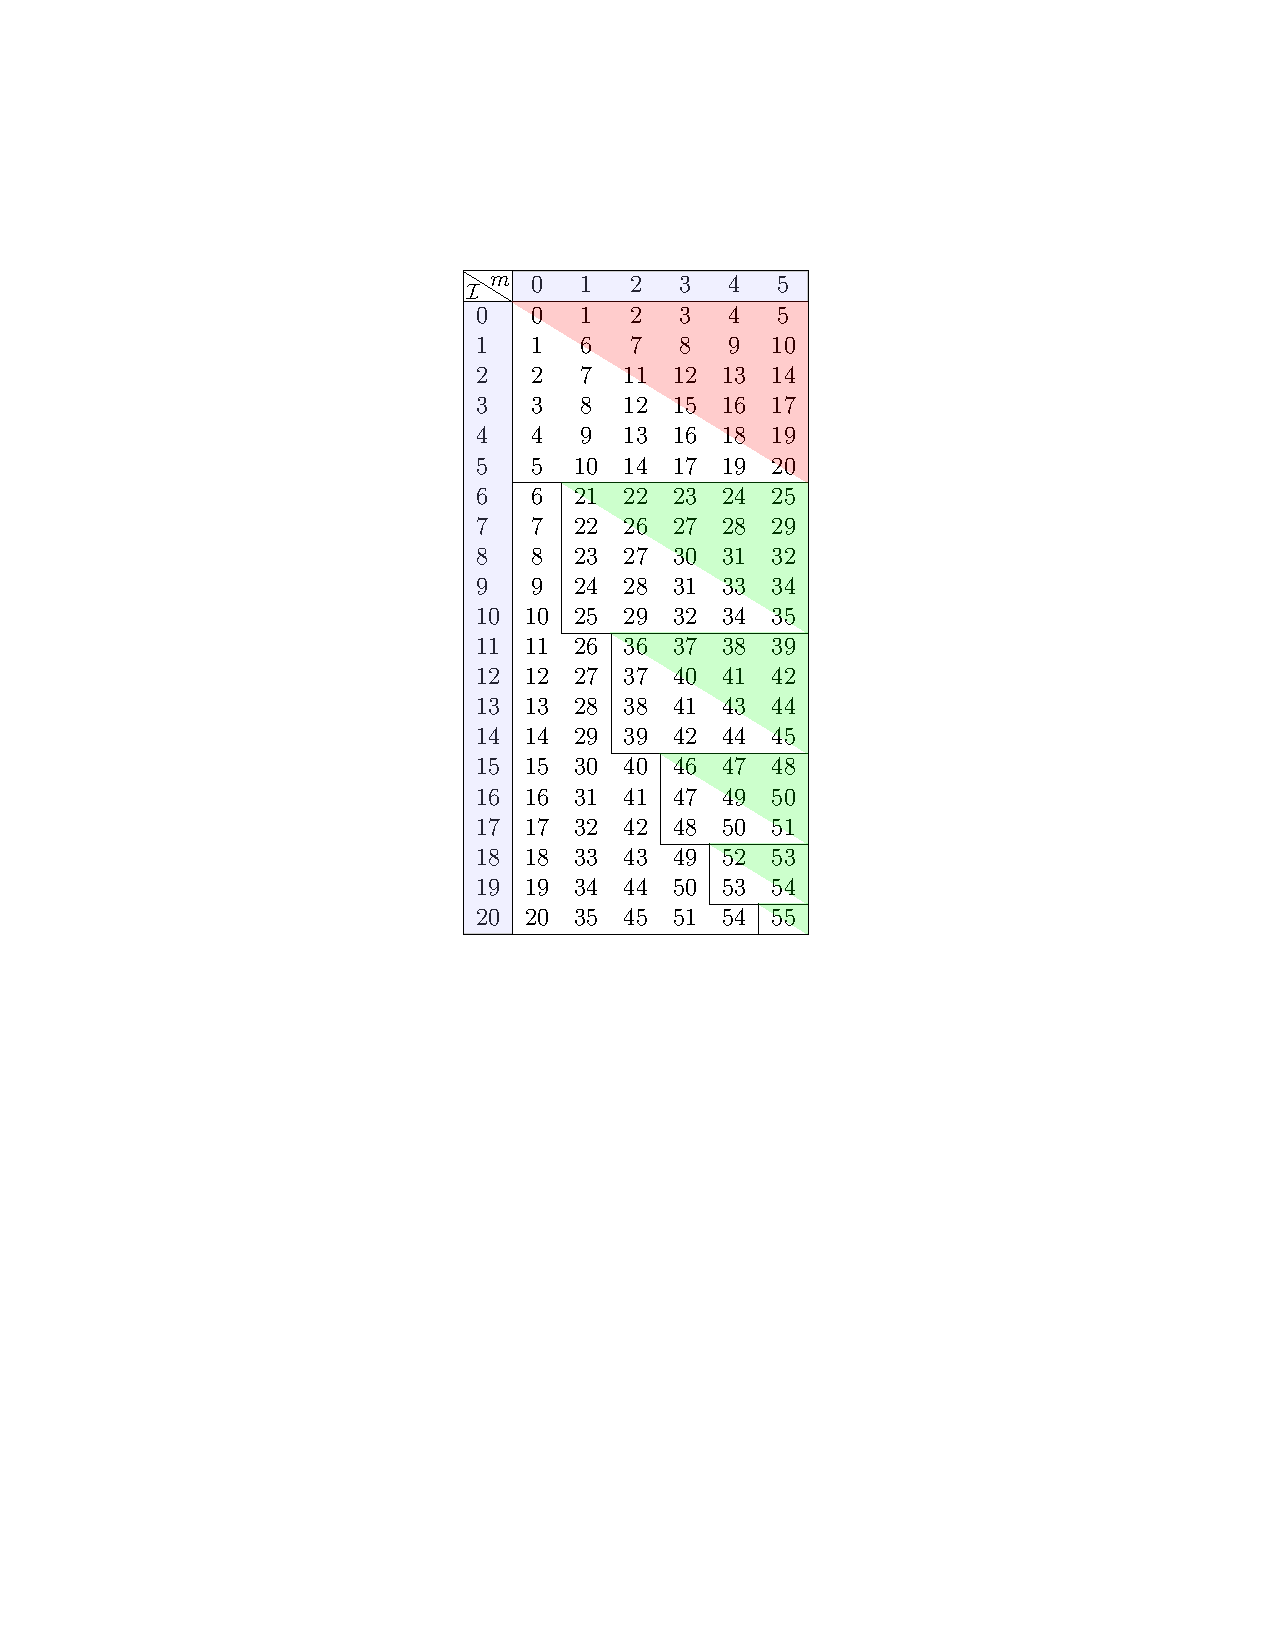
\includegraphics[width=0.55\columnwidth]{fig-map}
%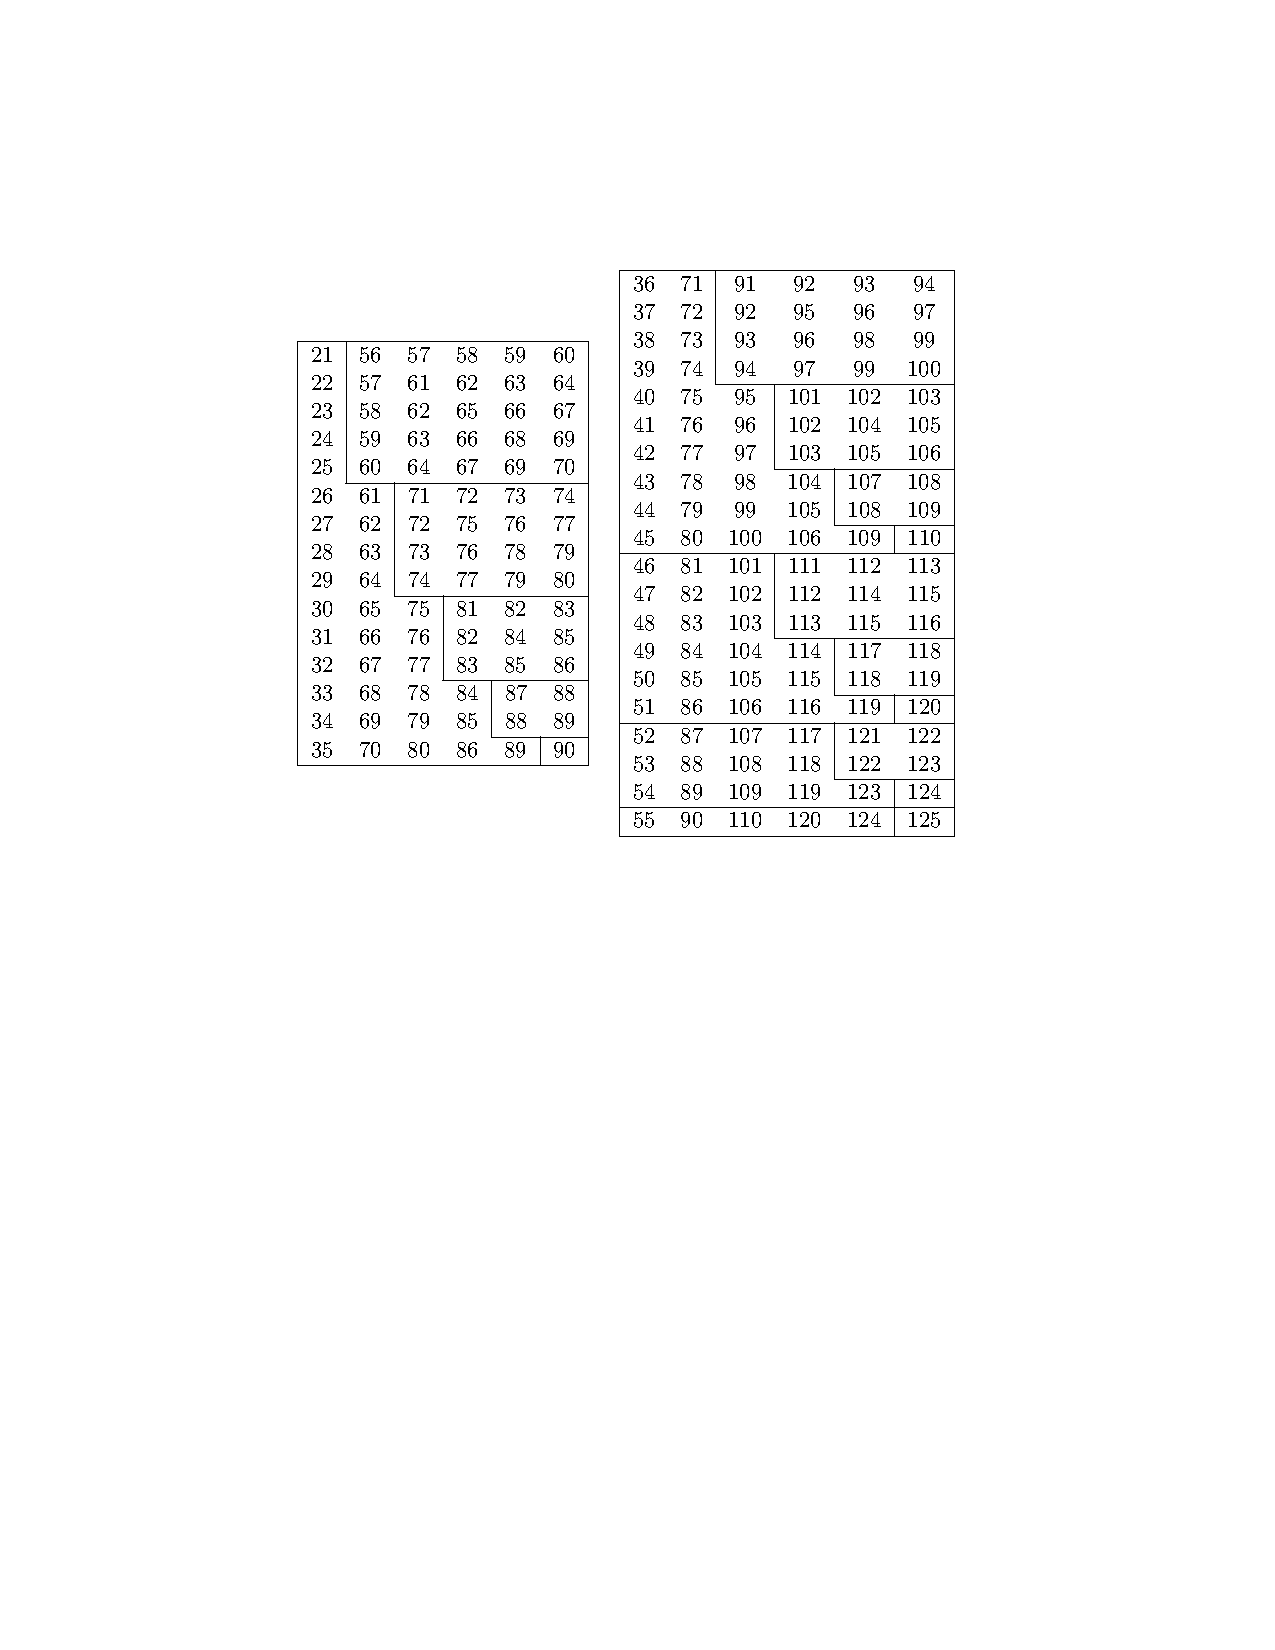
\includegraphics[width=0.5\columnwidth]{fig-table-n-4}
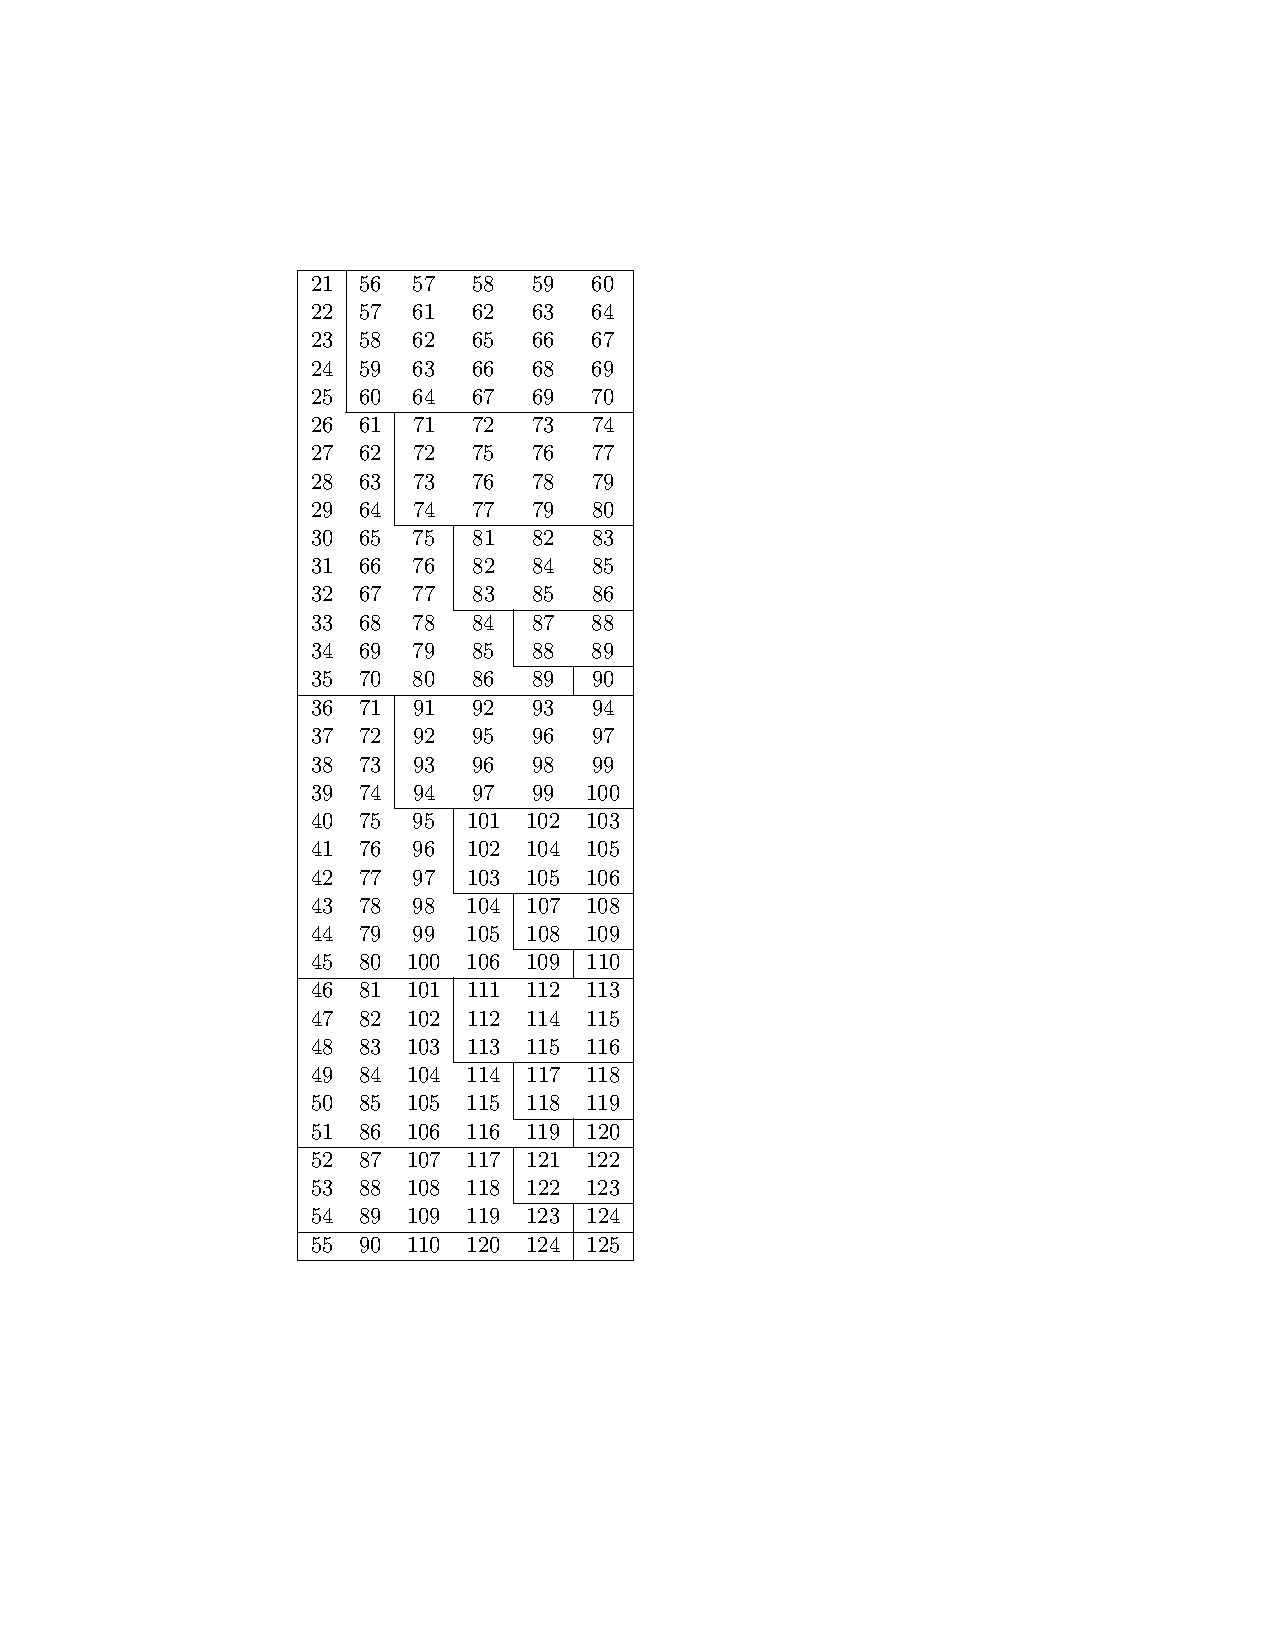
\includegraphics[width=0.35\columnwidth]{fig-n-4-1col}
\caption{  Map for N=3, M=5.
The map can be divided into two blocks, rows $0-5$ and $6-20$.
The second can be generated with a recursive function of depth $5$.
 \label{fig:map}
 }
\end{figure}

\subsection{Linear scaling calculations of the map $\maptoN$}
\subsubsection{Recognising the pattern}
If we represent the mappings for a fixed M, say $M=5$, and $N=2,3,4,5$,
as $2d$ arrays with
the indices of (N-1) sites basis 
and occupation number of Nth site as the
 row and column indices, and the indices of N sites basis as array elements,
we observe a clear recursive pattern with some symmetries. 
The map for N sites can be divided in blocks corresponding to addition of each site,
and each block consists of a series of square transpose-symmetric sub-blocks
 with sizes following a recursive pattern. 
To illustrate this, the mapping for $N=3$ and $M=5$ is shown in Fig.\ref{fig:map}. % with intentional shading of certain regions.
Here, rows $0-5$ make complete map for $N=2$.
 and there is a series of smaller sub-blocks in the second block, i.e., rows $6-20$.
To generate this map, we can divide it into these two blocks. 
The first block is simple to generate.
 If we see the red shaded triangular region, 
 we find that the index simply starts from 0 on the top left, 
 increases one by one as we move to the right, and leaves $i$ column for the $ith$ row
  due to the condition that the occupation for the second site should not be less than that of the first one.
The pattern gets a little complicated in the second block, rows $6-20$. First, see the green shaded regions.
These are a set of triangles with smaller and smaller sizes, 
again due to the restriction on the occupation of the third site.
These shaded regions are the part of the map that can be recorded when the basis are formed.
%The actual problem is to calculate the unshaded map. 
Our main task is to calculate the unshaded part of the map.
The pattern that the unshaded regions follow is also easy to see, however. 
In the first block, it's simply the symmetric image of the upper triangular part.
In the second block, 
the lower triangular parts of the square blocks around the recursion of triangles follow the same rule. 
The one extra complication is the columns on the left side not included in the square regions, but, 
they also follow a regular pattern. 
The first column starting from the row $6$ continues the count of the first column from the first block
 until the end of the second block.
 The other columns starting from row $11,15,18,19,20$, follow the same rule.

The depth of the recursion for the triangles in the figure for $N=3$ is $d=5$.
For $N=4$, there are recursions of depth $5,4,3,2,1$ originating from this recursion of order $5$.
This is a general feature of the mapping --- for any $N$, there are recursions of order $d,d-1,d-2,...,1$
 for each recursion of order $d$ in $N-1$ case!
 




\subsubsection{Generating the pattern}
Generating the $N=2$ map is trivial. 
We will first describe here how the $N>2$ blocks can be generated
and then how we implement this in our code.
%\subsubsection{Description}
Starting with $N=3$ case shown in Fig.\ref{fig:map}, 
a recursive function can generate the second part of the map, i.e., rows $6-21$,
 taking $M=5$, the depth of the recursion $d=5$, initial index $i=21$, and the starting index of the column on the left $i_c = 6$ as inputs. 
For $N>3$, we have to generate recursions of lower order/depths that would require starting values for multiple columns on the left side, $M-d$ values for order $d$ recursion, to be specific. 

In summary,
we can divide the map into blocks corresponding to recursions of various orders
and a function can generate each block given the required starting indices 
and the recursion depth. % starting index for triangular series, set of starting indices for the leftover columns, and the depth of the recursion.

\subsubsection{Implementation}
% The map for two sites is directly calculated, while
% all blocks for more than two sites are divided into sub-blocks each corresponding to a full recursion of triangles. 
 %Then they 
 These blocks can be generated sequentially or in parallel, and combined with the block for two sites.
 The sequential implementation (function \texttt{getmap}) is simpler, as all the arguments of the recursive function 
 ---
 starting index for the first triangle, the depth of the recursion, and 
 the set of starting indices for the leftover columns 
  --- are available at each call. 
 However, 
 we use this only for small system sizes. 
 For larger systems, the code uses a parallel implementation (function \texttt{getmapp}).
  There are two points to consider for parallelisation. 
  First, the arguments of the recursive functions need to be calculated beforehand, and second, the workload needs to be distributed evenly between all processes.
%The function needs three key arguments,
%the starting index, the recursion depth, and the initial values of the columns not included in the square regions in the Fig.\ref{fig:map}.
%These are generated sequentially.
The arguments are calculated sequentially (by function \texttt{getmapargs}), starting from the set for the first function call and, 
using the information on how much the indices are going to advance in that call, calculating the arguments for the next function call. 
This is illustrated in Algorithm\,\ref{alg:arg}. 
To distribute the load evenly, 
we calculate the block sizes (heights, ($d(d+1)/2$ for a recursion of depth $d$) that every recursion would produce,
the list `sizes' in Algorithm\,\ref{alg:arg}.
Using this list, the total size among all processes can be evenly divided.
This way, different processes can have different number of function calls but the total workload determined by the total size of the map they produce is approximately the same.

 %and make blocks for parallelisation with each recursion weighted by its size. 
 %
 Since, we only fill in a grid with indices that are obtained by either adding an integer to another or just plain ranges of integers,
 this method does not just scale linearly with the basis size, the slope of the scaling is very small,
 which makes it computationally extraordinarily efficient.











 
\section{Hamiltonian}
\label{sec:ham}

The Hamiltonian of the model system is the following.
\begin{multline}
 \tilde H
  =
  \omega \ad \an
  +
  \sum_i \left[
    \omega_0 \hat \sigma^+_i \hat \sigma^-_i
    +
    \frac{\omega_R}{\sqrt{N}} 
    \left( \hat \sigma^+_i \hat a^{} + \hat \sigma^-_i \hat a^\dagger \right)\right.
    \\+\left.
    \omega_v \left(
      \hat b^\dagger_i \hat b^{}_i
      - 
      \lambda_0 \sigma^+_i \hat \sigma^-_i 
      ( \hat b^\dagger_i + \hat b^{}_i ) \right)
  \right].
\end{multline}
The cavity photon mode (annihilation  operator $\an$) is coupled 
to many molecules, labeled $i=1\ldots N$.  
Each molecule is described by two electronic states 
(Pauli operator $\hat \sigma_i$), and a (harmonic) vibrational
degree of freedom (annihilation operator $\bn_i$).  
The optimal vibrational coordinate is displaced by
 $\lambda_0$ between the ground and excited electronic states.  
The matter-light coupling is parameterized by the collective
Rabi splitting $\omega_R$.

We displace the vibrational basis with the unitary transformation
$H = \mathcal{D}^\dagger(\lambda)\tilde H\mathcal{D}(\lambda)$,
where 
$\mathcal{D}(\lambda)=\exp[-\lambda\sum_{i=1}^N{(\bd_i-\bn_i)}]$ is the vibrational
displacement operator. [\az {check the sign of lambda/daggar on left or right}]
This gives %the following additional terms in the Hamiltonian.

\begin{multline}
  \label{eq:dh}
 H
  =
  \omega \ad \an
  +
  \sum_i \left[
    \omega_0 \hat \sigma^+_i \hat \sigma^-_i
    +
    \frac{\omega_R}{\sqrt{N}} 
    \left( \hat \sigma^+_i \hat a^{} + \hat \sigma^-_i \hat a^\dagger \right)
   \right.
        \\+\left.
        \omega_v
      \hat b^\dagger_i \hat b^{}_i +
     \omega_v( \lambda_0 \sigma^+_i \hat \sigma^-_i 
       - \lambda )( \hat b^\dagger_i + \hat b^{}_i )
   \right]
   - \omega_v\lambda(2\lambda_0+ N\lambda).
\end{multline}

While it looks quite similar to the Hamiltonian in the undisplayed basis, 
it introduces an extra complication of computing the matrix elements of 
$(\hat b^\dagger_i + \hat b^{}_i)$ 
for the unexcited sites
between the basis states in both the photon and exciton sectors.
However, this is a tiny cost for a huge gain in
 exponentially lowering the basis size.
 This is because the basis size scales exponentially with
  the cutoff on the vibrational space, 
  and the displaced basis (for optimum displacement) reduces the cutoff required for convergence to a fraction.
  \az{fraction, close to half? , displaceemnt? for optimum displacement. be specific here after having the plots of cutoff reduction, etc.}

The function \texttt{hamilt()} in hamiltonian.py 
calculates the Hamiltonian.
It uses the multiprocessing module
to parallelise the calculations for various terms in the Hamiltonian.
The results as sparse matrices are stored as global variables.

\subsection{Diagonal Terms}
The terms $\ad \an$, $ \sum_i \hat \sigma^+_i \hat \sigma^-_i$ are diagonal in
the basis used, 
and have the value $0(1)$ or $1(0)$ respectively in the
photon(exciton) subspace.  The term $\sum_i \hat b^\dagger_i \hat b^{}_i$ is
also diagonal, and is given by $N_v(i)$ in the photon block,
and $m+N_v(i)$ in the exciton block, for the permutation symmetric basis with index $i$.
This, in absolute terms, means that they correspond to
$i$th element for photon block and 
$\na + m*\nb + i$ for the exciton block.
\az{define photon/exciton subspaces/sectors/block and $N_v$, $m$, $\na$ and $\nb$ somewhere....}
\az{define somewhere, how we name the basis, which are actual list of basis set, which are permutation symmetric basis, etc... sectors.}
 
\subsection{Matter-Light Coupling}

The matter-light coupling $H_{g}= \sum_i\left(\hat \sigma^+_i \hat a^{} + \hat \sigma^-_i \hat
    a^\dagger\right)$ is relatively complicated
    as this mixes the two sectors, which are labeled differently. 
We focus on the photon emission term, as the other term follows by
conjugation.  
We need to find 
%$\Bigl( \bra{P}\otimes\bra{\alpha}_V \Bigr) \sum_i \hat \sigma^-_i \hat a^\dagger \Bigl( \ket{X}\otimes\ket{m,\beta}_V \Bigr) \equiv O_{\alpha, m, \beta} $
$( \bra{P}\otimes\bra{\alpha}_V) \sum_i \hat \sigma^-_i \hat a^\dagger ( \ket{X}\otimes\ket{m,\beta}_V ) \equiv O_{\alpha, m, \beta} $.
In order for this not to vanish, the set of final occupations of basis $\alpha$ must
have an element equal to $m$ and the rest of the set equal to the occupations of basis $\beta$.
If this is true, then we have:
\begin{displaymath}
  O_{\alpha, m^\ast, \beta} 
  = 
  \frac{N \cntsetx(\beta) }{\sqrt{N \cntsetx(\beta) } \sqrt{\cntset(\alpha)}}
\end{displaymath}
where $\cntsetx(\beta)$ is the count of distinct permutations as defined
%above.  
in \az{sectionXXX, $\alpha=\mathcal{M}(\beta,m^\ast) $}.
The factors $\sqrt{N \cntsetx(\beta)}$ and
$\sqrt{\cntset(\alpha)}$ in the denominator come from the normalization
of $\ket{m,\beta}_V$ and $\ket{\alpha}_V$.
The factors in the numerator come from the distinct ways in which
the overlap may occur --- a choice of $N$ molecules that may be excited, and
$\cntsetx(\beta)$ ways of arranging the unexcited molecules in the overlap.

Which combinations of $\alpha$, $m$, and $\beta$ will contribute, 
is exactly the information that the mapping $\maptoN$ contains.
So, we know a priory the right combinations to compute the non-zero matrix elements.
This helps save time by only computing the non-zero matrix elements.
The parallelisation is done over $\beta$ in this case that the mapping takes as one input.
A pseudocode for the function \texttt{getHg} that calculates the light-matter coupling term is presented in Algorithm\,\ref{alg:hg}.



\subsection{Vibrational Coupling}

The term coupling the electronic and vibrational states in the displaced basis is,
$H_{\lambda}=(\lambda_0 \sigma^+_i \hat \sigma^-_i - \lambda )( \hat b^\dagger_i + \hat b^{}_i )$. 
If the basis were not displaced, this term would have non-zero matrix elements
only in the exciton sector and diagonal in the permutation symmetric basis states for the unexcited molecules.
In the displaced basis,
we also need to evaluate the matrix elements of
$( \hat b^\dagger_i + \hat b^{}_i )$ for unexcited sites
in both the exciton and photon sectors.
However, using the mapping 
$\maptoN(\beta,m)$ and $\maptoNa(\gamma,m)$
simplifies the job.
We split the work in three parts.
The function \texttt{fHb} calculates the matrix elements for the excited site
whereas the functions \texttt{fHb1} and \texttt{fHb2}
do it for unexcited sites in photon and exciton sectors.





\subsubsection{Function \texttt{fHb}}
For states involving $\ket{X}_i$, it is
diagonal in the vibrational state of the other $N-1$ molecules $\beta$, and
so takes the form:
\begin{displaymath}
\bra{m^{\prime},\beta}_V( \hat b^\dagger_i + \hat b^{}_i )\ket{m,\beta}_V= \sqrt{m^{\prime}} \delta_{m-1,m^{\prime}}+ \sqrt{m}\delta_{m,m^{\prime}-1}
\end{displaymath}
where $m$ and $m^{\prime}$ are vibrational occupations of the excited
molecule. 
The evaluation of this is illustrated in Algorithm\,\ref{alg:hb}.

\subsubsection{Function \texttt{fHb1}}
For states involving $\ket{P}$,
we need to find which two states with indices
$\alpha$ and $\alpha^\prime$ reduce to the same 
$\beta$ for two consecutive single site occupations.
These give non-zero matrix elements of
$( \hat b^\dagger_i + \hat b^{}_i )$.
Again, the function \texttt{fHb1} simply uses $\maptoN$.
to determine required
$\alpha$ and $\alpha^\prime$ for a given $\beta$
and single site occupations $m$ and $m+1$.
The matrix element is
\begin{multline}
\bra{\alpha}_V( \hat b^\dagger_i + \hat b^{}_i )\ket{\alpha^\prime}_V= -\lambda N\sqrt{m}
\\ \times
\cntsetx(\beta) /\sqrt{\cntset(\alpha)\cdot \cntset(\alpha^\prime)}
\end{multline}


The implementation of this is illustrated in Algorithm\,\ref{alg:hb1}.


\subsubsection{Function \texttt{fHb2}}
This function computes the matrix elements of
$( \hat b^\dagger_i + \hat b^{}_i )$
for the unexcited sites in the exciton sector.
This term is diagonal in the excited site occupation,
but we have to pick one site from the N-1 unexcited sites
and, just like the \texttt{fHb1} case, find the basis states 
$\beta$ and $\beta^\prime$ that reduce to the same 
permutation symmetric basis state for N-2 sites
$\gamma$ when two consecutive single site occupations
 $m$ and $m^\prime=m+1$ are taken from the set of occupations they represent.


Similar to \texttt{fHb1}, \texttt{fHb2} uses the mapping $\maptoNa$
to determine required relationship 
$\beta$ and $\beta^\prime$ for a given $\gamma$
and single site occupations $m$ and $m+1$.
The matrix element is
\begin{multline}
\bra{\beta}_V( \hat b^\dagger_i + \hat b^{}_i )\ket{\beta^\prime}_V= -\lambda(N-1)\sqrt{m}
\\ \times \cntsetxx(\gamma) /\sqrt{\cntsetx(\beta)\cdot \cntsetx(\beta^\prime)}
\end{multline}
The implementation of this is illustrated in Algorithm\,\ref{alg:hb2}.





\section{Absorption}
\subsection{Transition matrix elements}
We wish to calculate the transition matrix elements $\bra{0} \hat a \ket{j}$
between the absolute ground state with no excitations of any kind and the eigenstates $\ket{i}$
of Hamiltonian in one excitation subspace (Eq.\,\ref{eq:dh}).
It is simple, but computationally very costly,
 both in terms of memory and processing,
because we need to compute
all eigenstates of the Hamiltonian that has very large dimensions,
which, in contrast to the Hamiltonian, are dense arrays.
However,
luckily, the matrix elements decay rapidly for transitions 
of energy more than a few $\omega_c$
so
we can select a low energy subset of
the spectrum. 
It is still very demanding for large system sizes so we recommend
 its usage should be limited to small systems.

\subsubsection{Function \texttt{fmatelem}}

This function calculates the eigenstates and then the transition matrix elements
which are just their $0$th components.
The eigenstates are calculated using the function
\texttt{fdiagl} or \texttt{fdiagw} in eigsolver.py, which
use function \texttt{lobpcg} from open source python library `scipy' \cite{scipy}
that implements an efficient iterative diagonalisation scheme \cite{lobpcg}.
The function \texttt{fmatelem} also calculates the cosine of the Hopfield angle,
 i.e., the photon fractions the eigenstates, 
 which is just the sum of absolute squares of 
 the coefficients of eigenstates in the photon sector.
 The matrix elements and photon fractions are written in output files
 `absoprtion.txt' that can be used later to calculate the absorption
  for desired cavity and exciton decay rates using the utility script
  absorption.py.
  


\subsection{Time evolution} %Two-time correlation}
The absorption spectrum can be obtained by 
taking the Fourier transform of two-time correlation 
$G(t) = \bra{0} \hat a(t)a^\dagger(0) \ket{0}$
\begin{displaymath}
G(\omega) = \int_0^\infty{G(t) e^{i\omega t} dt}.
\end{displaymath}
$G(t)$ is calculated as follows.

First, the initial state $\ket{\Psi(0)}$ is computed in the displaced basis.
Second,
the time dependent 
Schr\"{o}dinger equation is numerically integrated
to obtain $\ket{\Psi(t)}$
\begin{displaymath}
\ket{\Psi(t)} = \int_0^t { (H+H_{decay})\ket{\Psi(t^\prime)} dt^\prime},
\end{displaymath}
where, 
a non-hermitian term $H_{decay}$ is added to the Hamiltonian 
to include the cavity and exciton decay rates
$\kappa$ and $\gamma$.
It is $H_{decay} = i (\kappa \hat P_{photon} + \gamma \hat P_{exciton}) $, where $ \hat P_{photon}$ and $ \hat P_{exciton}$ are the projectors to the photon and exciton sectors.
Finally, $G(t)$ is obtained by the inner product
$G(t) = \bra{\Psi(t)}\ket{\Psi(0)}$.
This is repeated for $t$ on a grid of discretised time with long enough final time so that all relevant frequencies are captured in the correlation or the correlation decays to 
zero. 

The Fourier transform $G(\omega)$ is calculated once we have $G(t)$.
This is done by the function \texttt{getFourierTransform}.
Instead of using popular Fast Fourier transform routines,
we simply implement standard summation formula
so that we can compute the transform in a desired frequency window
and on a desired dense grid. 
This does not compromise any computational efficiency
because it involves relatively small grid sizes on time and frequency axes, $\sim 10^3$ and $\sim 10^2$, respectively.
$G(\omega)$ is written in the output file 
`abs-vs-w.txt' along with an analytical approximation \cite{cwik} to the same.


In the following, we will describe how the initial state $\ket{\Psi(0)}$ is calculated.

\subsubsection{The initial state}
The initial state for the time evolution is $\ket{\Psi(0)}=a^\dagger(0) \ket{0}$, i.e.,
the state with a photon but no exciton or vibrational quanta.
However, since we use vibrationally displaced basis states,
the vibrational part of our starting state is a multidimensional coherent state
\begin{displaymath}
\ket{\Psi(0)}=a^\dagger(0)\mathcal{D}(\lambda)\ket{0},
\end{displaymath}
with $\mathcal{D}(\lambda)=\exp[-\lambda\sum_{i=1}^N{(\bd_i-\bn_i)}]$
being the vibrational
displacement operator.
This multidimensional coherent state can be written as
\begin{displaymath}
\mathcal{D}(\lambda)\ket{0}_V = e^{-N\lambda^2/2}\sum_\alpha{\cntset(\alpha)\cdot\lambda^{N_v(\alpha)}/\sqrt{f(\alpha)}}\ket{\alpha}_V,
\end{displaymath}
where
$f(\alpha) = i_1! i_2!...i_N!$ is the product of factorials of 
the occupation numbers $\{i_1,i_2,...,i_N\}$ for the state $\ket{\alpha}_V$.
To handle expectedly large integers in the array $f$ with precision, 
we use opensource package `decimal' \cite{decimal}. 
$f$ is calculated by the function \texttt{fbasis} in basis.py and stored as a global array for later use by
the function \texttt{createpsi0}. 
%in correlation.py.

\az{should i include details that should go in `user manual'??, e.g., file names, function names?}





\section{Lower polariton state}

The function 
\texttt{gssolve} in gssolver.py
calculates the
lower polariton eigenstate using \texttt{lobpcg}
in functions 
\texttt{fdiagl} or \texttt{fdiagw}
in eigsolver.py.
We choose \texttt{lobpcg} over 
simple Arnoldi method or it's shift-invert version \cite{arnoldi} because it
can handle large system sizes $\sim 10^8$ relatively easily.
To make the Hamiltonian positive definite as required by \texttt{lobpcg},
it is shifted by it's lower bound
\begin{displaymath}
E_{LB}=(\omega_c+\omega_x-\omega_v \lambda_0^2)/2
-\sqrt{(\omega_c+\omega_x-\omega_v\lambda_0^2)^2 + \omega_R^2},
\end{displaymath}
which is obtained by replacing 
$\omega_x$ with
$\omega_x-\omega_v \lambda_0^2$
in 
the lower polariton's
energy
\begin{displaymath}
E_{LP}=(\omega_c+\omega_x)/2-\sqrt{(\omega_c+\omega_x)^2 + \omega_R^2}.
\end{displaymath}

In the following, we describe how the conditional density matrices are calculated.

\subsection{Conditional density matrices}

For our model, in subspace with a single conserved excitation,
i.e.,
$\ad \an+ \sum_i \hat \sigma^+_i \hat \sigma^-_i = 1$,
we can define three conditional reduced vibrational states
for a molecule.
{ \it(i) when there is a photon is the system}, $\ket{P}$,
{ \it(ii) when the molecule is electronically excited}, $\ket{X}_i$, and, 
{ \it(iii) when 
another molecule is electronically excited}, $\ket{X}_{j\neq i}$.
We calculate the upper triangular parts of these density matrices 
as describe in the following,
and obtain the rest from the hermitian symmetry.

\subsubsection{$\rho^{\ket{P}}$, when there is a photon is the system}
To find the element $\rho^{\ket{P}}_{m,m^\prime}$, we need to find all pairs
of states with indices
$\alpha,\alpha^\prime$
of the $N$ molecule problem which are reduced to the same $N-1$
molecule state with index $\beta$ when $m,m'$ are taken out
of their sets of occupations.
This is so that we can trace over $\beta$, the state of
the other molecules.
The matrix elements are given by
\begin{equation}
  \label{eq:rho0}
  \rho^{\ket{P}}_{m,m'} = \sum_{\beta=1}^{\nb}
  \frac{\psi^\ast_{P}(\alpha) \psi^{}_{P}(\alpha^\prime) \cntsetx(\beta)
  }{\sqrt{\cntset(\alpha) \cntset(\alpha^\prime)}},
\end{equation}
where
$\psi_P$ is the lower polariton eigenstate in $\ket{P}$ subspace.
The implementation of this in the code
parallelises the summation with the
summand calculated as illustrated in Algorithm \ref{alg:rho0} by
a function called \texttt{getrho0}. 



\subsubsection{$\rho^{\ket{X}_i}$, when the molecule is electronically excited}
\label{sec:rho1}

The calculation of $\rho^{\ket{X}_i}$ is simple because the state of the excited site is 
explicitly describe and the trace over the other $N-1$ sites is simple.

\begin{equation}
  \label{eq:reduce_Xi}
  \rho^{\ket{X}_i}_{m,m'} = 
  \frac{1}{N}
  \sum_{\beta=1}^\nb
  \psi^\ast_{X}(m,\beta)  \psi^{}_{X}(m^\prime,\beta)  
\end{equation}
Here $\psi_{X}(m,\beta)$ stands for the coefficient of the state with index
$(m\cdot \nb+ \beta)$ in the $\ket{X}$ subspace part of the lower polariton state,
 and the factor of $N$ appears
from the normalization of basis states.
Again, the implementation of this in the code
parallelises the summation.
The summand is calculated by 
a function \texttt{getrho1} as
illustrated in Algorithm \ref{alg:rho1}.




\subsubsection{$\rho^{\ket{X}_{j \neq i}}$, when another molecule is electronically excited}

To calculate $\rho^{\ket{X}_{j \neq i}}$, the conditional reduced density
matrix corresponding a different molecule being electronically excited,
we must trace over the excited molecule, and over $N-2$ of the $N-1$
unexcited molecules.  This is similar to the case for
$\ket{P}$, but this time we must use the mapping
$\maptoNa$, from the index $\gamma$ of distinct patterns of $N-2$ 
molecules and pairs of occupations for an unexcited site $m,m^\prime$
to the indexing $\beta,\beta^\prime$ of $N-1$ molecules.

\begin{multline} 
  \rho^{\ket{X}_{j \neq i}}_{m,m'} = 
   \sum_{m^{\ast}=0}^{M}
  \sum_{\gamma=1}^{\nc}
  \psi^\ast_{X}(m^\ast, \beta) \cdot
  \psi_{X}(m^\ast, \beta^\prime)
  \\ \times
  \frac{(N-1)\cntsetxx(\gamma)}{%
    N\sqrt{\cntsetx(\beta) \cntsetx(\beta^\prime)}},
\end{multline} 
where
$\beta = \maptoNa(m, \gamma)$, $\beta^\prime = \maptoNa(m^\prime, \gamma)$,
and $\psi_{X}(m,\beta)$ have the same meaning as in section\,\ref{sec:rho1}.
The summation over the $\gamma$ is parallelised over in the code
 with a function \texttt{getrho2} with structure similar to that of \texttt{getrho0}
 with an extra summation over the occupation of the excited site.



\section{Input file}

The following variables need to be defined in the input file
to describe the system and type of calculations desired.

\subsection{system specification}

\begin{comment}

\begin{description}
\itemsep 5pt
\parsep 0pt

\item[{\bf NumberOfSites}]({\it integer}):
An integer or a list of integers specifying the number of molecules in the system.\\
Examples: NumberOfSites = 4, NumberOfSites = [1,3,5].\\
{\it Default value:} 2 

\item[{\bf VibrationalCutoff}]({\it integer}):
An integer or a list of integers specifying the maximum number of vibrational quanta per site.
Examples: VibrationalCutoff = 5, VibrationalCutoff = [5,5,3].\\
\end{description}
{\bf NumberOfSites}:
\end{comment}


The number of molecules $N$ is specified 
as a single integer with variable \texttt{n},
 or a list of integers for a set of system sizes
 with variable \texttt{nlist}.
The cutoff on the vibrational levels, $M$,
is specified by a variable
\texttt{m}.
If \texttt{nlist} is given,
a corresponding \texttt{mlist} can also be given
 to use different cutoffs for different system sizes.

The values of $\omega_c,\omega_x,\omega_v,\omega_R$, and $\lambda_0$
are specified by the variables
\texttt{wc,wx,wv,wr}, and \texttt{lambda0}, respectively.


\subsection{Type of calculations}
Two basic types of calculations correspond to
ground state (default) and absorption.
For the ground state calculations, 
a string \texttt{onlyenergy=`true'} in the input can be given 
to calculate only the lower polariton energy and
leave the conditional density matrices.

Absorption is calculated when 
a string \texttt{absorption=`true'} is given in the input file.
By default, matrix elements are calculated. 
The number of low energy states can be limited by an integer variable 
\texttt{nstates}.
If another string \texttt{td=`true'} is given, the time evolution
is performed and two-time correlation and its Fourier transform
are calculated. 
For this, the following variables should be provided.
The decay rates of
cavity and exciton 
as variable \texttt{kappa} and \texttt{gamma},
time evolution related variables,
final time as \texttt{tf}, 
time interval for correlation data as \texttt{dt},
the boundaries of frequency window (relative to the bare exciton line)
as \texttt{e1,e2}, and the number of points on this window as \texttt{nwft}.

For any type of calculation, 
a range of values for coupling constants 
$\omega_R$ or $\lambda_0$
can be given with total number of points 
and the code would iterate over it in the best possible way.
These are specified by the variables
\texttt{wmin, wmax}, and \texttt{nwmax} with a string variable 
\texttt{loopover =  `wr'}, or \texttt{lmin, lmax}, and \texttt{nlmax} 
with \texttt{loopover = `lambda0'}.

\subsection{Parallelisation}
The number of processes can be specified in the input file 
with a variable \texttt{Np}. 
However, some tasks utilise less processes. For example,
the parallelisation over the set of values of $\omega_R$ or $\lambda_0$
 uses only \texttt{nwmax} or \texttt{nlmax}
processes if these are less than \texttt{Np}.

\subsection{Output}
Output is saved in a directory `data'.
By default,
the energy and density matrices files from ground state calculations
are saved in a subdirectory `n-[{\it number of molecules}]',
and absorption output files for matrix elements or $G(t)$ and $G(\omega)$
are written in a single file for all number of molecules in \texttt{nlist}.
A variable \texttt{diffoutdir = 1 or 0}, specifying if 
different output directories should be used or not,
can change this behaviour.

\subsection{Convergence of diagonalisation}
The maximum number of iterations for the diagonalisation
 and the tolerance for convergence can be specified with variables
\texttt{itermax} and \texttt{tolr}.





%ld & float & fraction of $\lambda_0$ the basis are displaced & ld = 0.5\\ 
%diffoutdir & integer 0/1 & seperate output directories for different number of molecules & 












\begin{displaymath}
\end{displaymath}


\vspace{2cm}

\begin{comment}
The map can be divided in blocks that can be generated with recursive functions (or different orders/levels).
In this figure, the row 6-20 is a block of order 5. If we know the starting value of the running index (21), and the starting value of the column on the left (6), we can create this block. 
For n=4, there are 5 such blocks, or order 5,4,3,2,1, needing increasing number of starting values for the columns on the left.
For large n, the same pattern repeats, making a set of lower and lower order/rank blocks for every block in the previous n sector.
That is, for n=3, iarg = [5], for n=4, it's [5,4,3,2,1], for n=5, it's [5,4,3,2,1,4,3,2,1,3,2,1,2,1,1], and so on....
How to parrelise? predetermine iarg, karg, and cols. (also availability of sizes list will help allocate the arrays of right size, etc.), how to evenly distribute the workload.......
\end{comment}


 



 \vspace{2cm}



\az{
There is a bottleneck of using the permutation symmetry for this problem. For calculating the matrix elements of light-matter coupling term in the Hamiltonian
(and also for calculating the conditional vibrational density matrices), 
we need to evaluate the inner products of vibrational basis states
that are permutation symmetric in different number of sites.
In photon sector, all sites are equivalent so the basis states are N-symmetric,
 whereas, in the exciton sector, they are (N-1)-symmetric, with the electronically excited site explicitly described.
Thus, a mapping is needed that tells us which N-symmetric
basis state can have non-zero overlap with which pair of
(N-1)-symmetric basis and state for (electronically) excited site.
A naive way of calculating this map is to compare the sets of occupation numbers of these states but this scales badly ($\sim N_s^2$) with the number of permutation symmetric basis states and hence 
hugely reduces the potential of the method making it impractical for large systems.




Algorithm:
Implementation:
How to find the mappings? formula????
Displaced basis
extra basis

minor details:
lower bound for positivitiy, lobpcg
eshift for detuning=0,

corrtf: displaced basis, psi0 construction/computation from Hphot
matrix elem: postprocessing with desired decay rates

loop over coupling parameters: lambda0/wr
several N,M,Mx in a single run

input format
output formats
utils
wigner functions
absorption from matrix elem
analytic green function

implementation:
how basis are formed, what to retain for later use: norms, Nvs, map, factlist

performance
scaling
mem/time

tutorials
examples

manual
download
install/build executable or run the scrip main.py using python.


some algorithms
"efficient implementation"

}




































\begin{thebibliography}{0}
\bibitem{1}Reference 1         % This list should only contain those items referenced in the                 
\bibitem{2}Reference 2         % Program Summary section.   
\bibitem{3}Reference 3         % Type references in text as [1], [2], etc.
                               % This list is different from the bibliography at the end of 
                               % the Long Write-Up.
\end{thebibliography}
* Items marked with an asterisk are only required for new versions
of programs previously published in the CPC Program Library.\\
\end{small}


%% main text
\section{}
\label{}

%% The Appendices part is started with the command \appendix;
%% appendix sections are then done as normal sections
%% \appendix

%% \section{}
%% \label{}

%% References
%%
%% Following citation commands can be used in the body text:
%% Usage of \cite is as follows:
%%   \cite{key}         ==>>  [#]
%%   \cite[chap. 2]{key} ==>> [#, chap. 2]
%%

%% References with bibTeX database:

\bibliographystyle{elsarticle-num}
\bibliography{<your-bib-database>}

%% Authors are advised to submit their bibtex database files. They are
%% requested to list a bibtex style file in the manuscript if they do
%% not want to use elsarticle-num.bst.

%% References without bibTeX database:

% \begin{thebibliography}{00}

%% \bibitem must have the following form:
%%   \bibitem{key}...
%%

% \bibitem{}

% \end{thebibliography}



\onecolumn



\renewcommand{\theequation}{S\arabic{equation}}
\setcounter{equation}{0}
\renewcommand{\thefigure}{S\arabic{figure}}
\setcounter{figure}{0}
\setcounter{section}{0}

\clearpage

%\onecolumngrid
\begin{center}
\textbf{\large Supplemental Material: Polaritons code}

\vspace{0.4cm}

{M.\ Ahsan Zeb, Peter G.\ Kirton and Jonathan Keeling} \\
\textit{SUPA, School of Physics and Astronomy, University of St Andrews, St Andrews, KY16 9SS, United Kingdom}\\
(Dated: \today)

\end{center}
\vspace{\columnsep}
%\twocolumngrid

This supplemental material provides further details of the polynomial-scaling
algorithm used to exactly solve the Holstein--Tavis--Cummings model....





\begin{algorithm}
  \caption{Arguments for recursive function \texttt{trianglesp}}\label{alg:arg}
\begin{algorithmic}[100]
    \Function{getmapargs}{$N,M$} 
          \State {\it\color{brown}{$\diamond$ initialise output lists}}   
         \State	$ind_{tri} = [\,]; depth_{rec} = [\,]; ind_{col} =[\,]; sizes = [\,];$
      \State {\it\color{brown}{$\diamond$ initial arguments (for $n=3$ block) }  }
      	\State	$indtri = (M+1)(M+2)/2 - 1$ \Comment{index for triangular recursion}
      	\State	$depths = [M]$  \Comment{recursion depth}
      	\State	$indcols = np.array([M])$ \Comment{index for column}
      \State {\it\color{brown}{$\diamond$ iterations over sites and recursions}  } 
    \For{\texttt{$n$ in range($3,N+1$)}}
          	\State	$depths_{aux} = [\,]$\Comment{to temporarily hold depths for next $n$}
        \For{\texttt{$d$ in $depths$}}
     \State {\it\color{brown}{$\diamond$ take only the first $M-d$ columns, discard the rest, if any.}}
     % \State {\it\color{brown}{$\diamond$ reset $indcols$ to its first $M-d$ elements}}
       \State \texttt{$indcols = indcols[0:M-d+1]$}\Comment{desired reseting}
       \State {\it\color{brown}{$\diamond$ block height (number of rows) for current recursion}} 
        \State \texttt{$h= d(d+1)/2$}
       \State {\it\color{brown}{$\diamond$append current values to the output lists}} 
       \State \texttt{Append $d$ to $depth_{rec}$} 
              \State \texttt{Append $indtri $ to $ind_{tri}$} 
                 \State \texttt{Append $indcols$ to $ind_{col}$} 
      \State \texttt{Append $h$ to $sizes$}
       \State {\it\color{brown}{$\diamond$ indices for the next iteration}}
       \State  $indcols = indcols + h$ \Comment{add $h$ to every element of indcols}
     	\State \texttt{Append $indtri+h$ to $indcols$}  \Comment{an additional column}
      \State $indtri   \pluseq d(d+1)(d+2)/6$\Comment{+ total `length' of triangles}
         \State {\it\color{brown}{$\diamond$ For every recursion of depth $m$ in current $n$,}}
         \State {\it\color{brown}{$d$ recursions of depth $d,d-1,...,1$ for the next n, i.e., $n+1$}}
      \State \texttt{$depths_{aux} \pluseq [d,d-1,d-2,...,1]$} %list(range($1,m+1$))[$::-1$]
              \EndFor 
       \State \texttt{$depths = depths_{aux}$} \Comment{depths for next $n$}
       \EndFor  
       \State \Return $ind_{tri}, depth_{rec}, ind_{col}, sizes$
\Comment{Output}
    \EndFunction
 \end{algorithmic}
\end{algorithm}





\begin{algorithm}
  \caption{Light-matter coupling term}\label{alg:hg}
  \begin{algorithmic}[1]
    \Function{getHg}{$\beta$}\Comment{The index of N-1 symmetric basis}
     \State \texttt{$H_g=[\,];$} \Comment{Start output as an empty list}
     \State \texttt{$m_2 = \cntsetx(\beta)$} \Comment{Permutations of $\beta$ state}
    \For{\texttt{$m$ in range(0,M+1)}} \Comment{Loop over single site occupations}
       \State \texttt{$j= \na + m\cdot \nb + \beta$} \Comment{Absolute index}
        \State \texttt{$\alpha = \maptoN(\beta,m)$}\Comment{$\alpha$ from mapping}
        \State \texttt{$m_1 = \cntset(\alpha)$;\, } \Comment{Permutations of $\alpha$ state}
        \State \texttt{$h=\sqrt{N\cdot m_2/m_1}$}\Comment{Matrix element}
        \State \texttt{Append $[\alpha,j,h]$ to $H_g$} \Comment{Append to the output list}
        \EndFor  
       \State \Return $H_g$\Comment{Output}
    \EndFunction
  \end{algorithmic}
\end{algorithm}
%\textbf{return} 



\begin{algorithm}
  \caption{Vibrational coupling, excited state term}\label{alg:hb}
  \begin{algorithmic}[1]
    \Function{fHb}{$\beta$}\Comment{The index of N-1 symmetric basis}
     \State \texttt{$H_b=[\,];$} \Comment{Start output as an empty list}
     \For{\texttt{$m$ in range(1,M+1)}} \Comment{Loop over single site occupations}
       \State \texttt{$j= \na + (m-1)\cdot \nb + \beta$} \Comment{Absolute index}
        \State \texttt{$j^\prime= \na + m\cdot \nb + \beta$} 
        \State \texttt{$h=(\lambda_0-\lambda)\sqrt{m}$}\Comment{Matrix element}
        \State \texttt{Append $[j,j^\prime,h]$ to $H_b$} \Comment{Append to the output list}
        \EndFor  
       \State \Return $H_b$\Comment{Output}
    \EndFunction
  \end{algorithmic}
\end{algorithm}



\begin{algorithm}
  \caption{Vibrational coupling, photon sector term}\label{alg:hb1}
  \begin{algorithmic}[1]
    \Function{fHb}{$\beta$}\Comment{The index of N-1 symmetric basis}
     \State \texttt{$H_b=[\,];$} \Comment{Start output as an empty list}
        \State \texttt{$m_2=\cntsetx(\beta) $} \Comment{Permutations of $\beta$ state}
     \For{\texttt{$m$ in range(1,M+1)}} \Comment{Loop over single site occupations}
      \State \texttt{$m^\prime=m+1$}
       \State \texttt{$\alpha = \maptoN(\beta,m)$}\Comment{$\alpha,\alpha^\prime$ from mapping}
      \State \texttt{$\alpha^\prime = \maptoN(\beta,m^\prime)$} 
         \State \texttt{$h= -\lambda\cdot m_2\cdot N\cdot\sqrt{m}/\sqrt{\cntset(\alpha)\cdot \cntset(\alpha^\prime)}$}\Comment{Matrix element}
        \State \texttt{Append $[\alpha,\alpha^\prime,h]$ to $H_b$} \Comment{Append to the output list}
        \EndFor  
       \State \Return $H_b$\Comment{Output}
    \EndFunction
  \end{algorithmic}
\end{algorithm}




\begin{algorithm}
  \caption{Vibrational coupling, unexcited sites in exciton sector}\label{alg:hb2}
  \begin{algorithmic}[1]
    \Function{fHb2}{$\gamma$}\Comment{The index of N-2 symmetric basis}
     \State \texttt{$H_b=[\,];$} %\Comment{Start output as an empty list}
        \State \texttt{$m_3=\cntsetxx(\gamma) $} \Comment{Permutations of $\gamma$ state}
     \For{\texttt{$m$ in range(1,M+1)}} \Comment{Loop over single site occupations}
      \State \texttt{$m^\prime=m+1$}
       \State \texttt{$\beta = \maptoNa(\gamma,m)$}\Comment{$\beta, \beta^\prime$ from mapping}
      \State \texttt{$\beta^\prime = \maptoNa(\gamma,m^\prime)$}
         \State \texttt{$h= -\lambda\cdot m_3\cdot (N-1)\cdot\sqrt{m}/\sqrt{\cntsetx(\beta)\cdot \cntsetx(\beta^\prime)}$}%\Comment{Matrix element}
              \For{\texttt{$m^\ast$ in range(0,M+1)}} \Comment{Loop over excited site state}
              \State \texttt{$j= \na + m^\ast\cdot \nb + \beta$}   \Comment{Absolute indices}
         	\State \texttt{$j^\prime= \na + m^\ast\cdot \nb + \beta^\prime$} 
	        \State \texttt{Append $[j,j^\prime,h]$ to $H_b$} \Comment{Append to the output list}

               \EndFor  
        \EndFor  
       \State \Return $H_b$\Comment{Output}
    \EndFunction
  \end{algorithmic}
\end{algorithm}




\begin{algorithm}
  \caption{$\rho^{\ket{P}}$, when there is a photon is the system}\label{alg:rho0}
  \begin{algorithmic}[1]
    \Function{getrho0}{$\beta$}\Comment{The index of N-1 symmetric basis}
     \State \texttt{$\rho_0 =$\, numpy.zeros($(M+1,M+1)$)} \Comment{initialise as a numpy array}
     \State \texttt{$m_2=\cntsetx(\beta)$}
     \For{\texttt{$m$ in range(0,M+1)}} \Comment{Loop over single site occupations}
       \State \texttt{$\alpha = \maptoN(\beta,m)$}
         \State \texttt{$m_1=\cntset(\alpha) $}
     \For{\texttt{$m^\prime$ in range(m,M+1)}} \Comment{Upper triangular of $\rho^{\ket{P}}$}
       \State \texttt{$\alpha^\prime = \maptoN(\beta,m^\prime)$} 
         \State \texttt{$m_1^\prime=\cntset(\alpha^\prime) $}
         \State $\rho_0(m,m^\prime) \pluseq  \psi(\alpha)^\ast \cdot \psi(\alpha^\prime) \cdot m_1/\sqrt{m_1\cdot m_1^\prime}$
       	\EndFor 
        \EndFor  
       \State \Return $\rho_0$\Comment{Output}
    \EndFunction
  \end{algorithmic}
\end{algorithm}





\begin{algorithm}
  \caption{$\rho^{\ket{X}_i}$, when the molecule is electronically excited}\label{alg:rho1}
  \begin{algorithmic}[1]
    \Function{getrho1}{$\beta$}\Comment{The index of N-1 symmetric basis}
     \State \texttt{$\rho_1 = $\,numpy.zeros($(M+1,M+1)$)} \Comment{Start output as a numpy array}
     \For{\texttt{$m$ in range($0,M+1$)}} \Comment{Loop over single site occupations}
         \State \texttt{$j = \na + m\cdot\nb + \beta $}     \Comment{Absolute index}
     \For{\texttt{$m^\prime$ in range($m,M+1$)}}
         \State \texttt{$j^\prime = \na + m^\prime\cdot\nb + \beta $}  
         \State $\rho_0(m,m^\prime) \pluseq  \psi(j)^\ast \cdot \psi(j^\prime) /N$
        \EndFor  
        \EndFor 
       \State \Return $\rho_1$\Comment{Output}
    \EndFunction
  \end{algorithmic}
\end{algorithm}





\begin{algorithm}
  \caption{$\rho^{\ket{X}_{j\ne i}}$,  when another molecule is electronically excited}\label{alg:rho2}
  \begin{algorithmic}[1]
    \Function{getrho2}{$\gamma$}\Comment{The index of N-2 symmetric basis}
     \State \texttt{$\rho_2 = $\,numpy.zeros($(M+1,M+1)$)} \Comment{Start output as a numpy array}
     \State \texttt{$m_3=\cntsetxx(\gamma)\cdot (N-1)/N$} 
     \For{\texttt{$m$ in range(0,M+1)}} \Comment{Loop over single site occupations}
       \State \texttt{$\beta = \maptoNa(\gamma,m)$}
         \State \texttt{$m_2=\cntsetx(\beta) $} 
     \For{\texttt{$m^\prime$ in range(m,M+1)}} \Comment{Upper triangular of $\rho^{\ket{X}_{j\ne i}}$}
              \State \texttt{$\beta^\prime = \maptoNa(\gamma,m^\prime)$}
         \State \texttt{$m_2^\prime=\cntsetx(\beta^\prime) $}
             \State $x = m_3/\sqrt{m_2\cdot m_2^\prime}$
       \For{\texttt{$m^\ast$ in range(0,M+1)}}
           \State \texttt{$j = \na + m^\ast\cdot\nb + \beta $}     \Comment{Absolute index}
            \State \texttt{$j^\prime = \na + m^\ast\cdot\nb + \beta^\prime $}                
         \State $\rho_2(m,m^\prime) \pluseq  \psi(j)^\ast \cdot \psi(j^\prime) \cdot x$
       	\EndFor 
	\EndFor 
        \EndFor  
       \State \Return $\rho_2$\Comment{Output}
    \EndFunction
  \end{algorithmic}
\end{algorithm}


























\begin{comment}
First, although trivial,
consider the absolute indices 
of full basis set to introduce some terminology.
We place the photon block before the exciton one.
For the photon block, the absolute index of the basis 
is the same as the index of the vibrational basis $\alpha$ for it.
However, for the exciton block, since the excited site is explicitly described, the absolute index for a given basis
is 
\begin{displaymath}
i=\na + m\cdot\nb + \beta,
\end{displaymath}
where $\na$ and $\nb$ are total number of permutation symmetric states in photon and exciton sectors, 
$m$ is the vibrational state for the excited site, and,
$\beta$ is the index of permutation symmetric basis state
in the exciton sector.
We will consistently use symbols $\alpha$ and $\beta$ to refer to the indices of the permutation symmetric states in the photon and exciton sectors. This will save us writing extra labels to specify these two sectors and also make various expressions more readable.
\end{comment}





\end{document}
